\documentclass[
    hyperref={
        final,
        colorlinks=true,
        menucolor=black,
        anchorcolor=green,
        linkcolor=blue,
        citecolor=red,
        pdftitle={RS RAS Internship Presentation},
        pdfauthor={Moritz M. Konarski}
    }
]{beamer}

\mode<presentation>
{
  \usetheme{Goettingen}
  \usecolortheme{seahorse}
  \usefonttheme{serif}
  \setbeamertemplate{navigation symbols}{}
  \setbeamertemplate{caption}[numbered]
}

\addtobeamertemplate{navigation symbols}{}{%
    \usebeamerfont{footline}%
    \usebeamercolor[fg]{footline}%
    \hspace{1em}%
    \insertframenumber/\inserttotalframenumber
}

\usepackage{amsmath}
\usepackage{amsfonts}
\usepackage{graphicx}
\usepackage{float}
\usepackage[english]{babel}
\renewcommand{\baselinestretch}{1.2}
\usepackage{textcomp}
\usepackage{chngcntr}
\counterwithin{figure}{section}

\makeatletter
\patchcmd{\@listI}{\itemsep3\p@}{\itemsep10pt}{}{}
\makeatother

\newcommand{\figref}[1]{\figurename~\ref{#1}}
\newcommand{\tabref}[1]{\tablename~\ref{#1}}

\newcommand{\makefig}[4]{                                                       
    \begin{figure}[#1]                                                          
        \captionsetup{justification=centering}                                  
        \includegraphics[width=#2]{#3}                                          
        \caption{#4}                                                            
        \label{fig:#3}                                                          
    \end{figure}                                                                
}

\AtBeginSection[]{
    \begin{frame}
        \vfill
        \centering
        \begin{beamercolorbox}[sep=8pt,center,shadow=false,rounded=false]{title}
            \usebeamerfont{title}\insertsectionhead\par
        \end{beamercolorbox}
        \vfill
    \end{frame}
}

\setbeamertemplate{frametitle}[default][center]
\setbeamertemplate{bibliography item}{\insertbiblabel}
 
\title[RS RAS Internship]{RS RAS Internship Report}
\author[M. Konarski]{Moritz M. Konarski}
\institute[AUCA]{Applied Mathematics Department \\
    American University of Central Asia}
\date{\today}

\begin{document}

\begin{frame}
  \titlepage
\end{frame}

\begin{frame}{Outline}
  \tableofcontents
\end{frame}

\section{Introduction}

\begin{frame}{Place of internship}
    \begin{itemize}
        \item Federal State Budgetary Institution of Science Research Station 
            of the Russian Academy of Sciences in Bishkek (RS RAS)
        \item employs 137 people
        \item founded in 1978
        \item researches seismic processes and develops geodynamic models
            \cite{rsras-website}
    \end{itemize}
\end{frame}

\begin{frame}{Educational internship tasks}
    \begin{enumerate}
        \item familiarize yourself with web resources providing access to NASA 
            Earth Remote Sensing data
        \item familiarize yourself with the scientific data format netCDF 
            (Network Common Data Form)
        \item study libraries used to work with the netCDF format in various 
            computing environments
    \end{enumerate}
\end{frame}

\begin{frame}{Industrial internship tasks}
    \begin{enumerate}
        \item register on the NASA Earthdata platform to access satellite data
        \item develop a library for working with netCDF files in the Python
            programming language (using satellite data as an example)
        \item develop a computer application for data visualization and 
            reanalysis of NASA MERRA--2 satellite data.
    \end{enumerate}
\end{frame}

\begin{frame}{The end product}
    \begin{itemize}
        \item a Python application with a graphical user interface that:
            \begin{itemize}
                \item extracts variables from netCDF files and saves them to NPZ 
                    files
                \item takes those NPZ files and selects subsets of their data
                \item either exports that data or plots that data
                \item data can be heat map or time series
            \end{itemize}
    \end{itemize}
\end{frame}

\section{The Data}

\begin{frame}{What data are we using?}
    \begin{itemize}
        \item NASA Modern-Era Retrospective analysis for Research and 
            Applications version 2 (MERRA--2)
        \item specifically
    \href{https://disc.gsfc.nasa.gov/datasets/M2I3NPASM_5.12.4/summary}{M2I3NPASM};
            Jan. 1, 1980 to Oct. 1, 2020
        \item covers whole globe, measurements every 3 hours \cite{data-summary}
        \item 14 variables with latitude, longitude, time, pressure level 
            \cite{data-readme}:
            \begin{itemize}
                \item surface pressure
                \item specific humidity
                \item temperature
            \end{itemize}
    \end{itemize}
\end{frame}

\begin{frame}[fragile]{Where do we get the data?}
    \begin{itemize}
        \item MERRA--2 data (M2I3NPASM) available at NASA Goddard Earth 
            Sciences (GES) Data and Information Services Center (DISC)
    \href{https://disc.gsfc.nasa.gov/datasets/M2I3NPASM_5.12.4/summary}{here}
        \item requires account \cite{earthdata-policy} but is free 
            \cite{esds-website}
        \item a subset of the data can be downloaded, see \figref{map}
        \item download is convenient using the command--line application 
        \href{https://disc.gsfc.nasa.gov/data-access#mac_linux_wget}{wget}
    \end{itemize}
\end{frame}


\begin{frame}{Data subset}
    \begin{figure}[H]
        \center
        \fbox{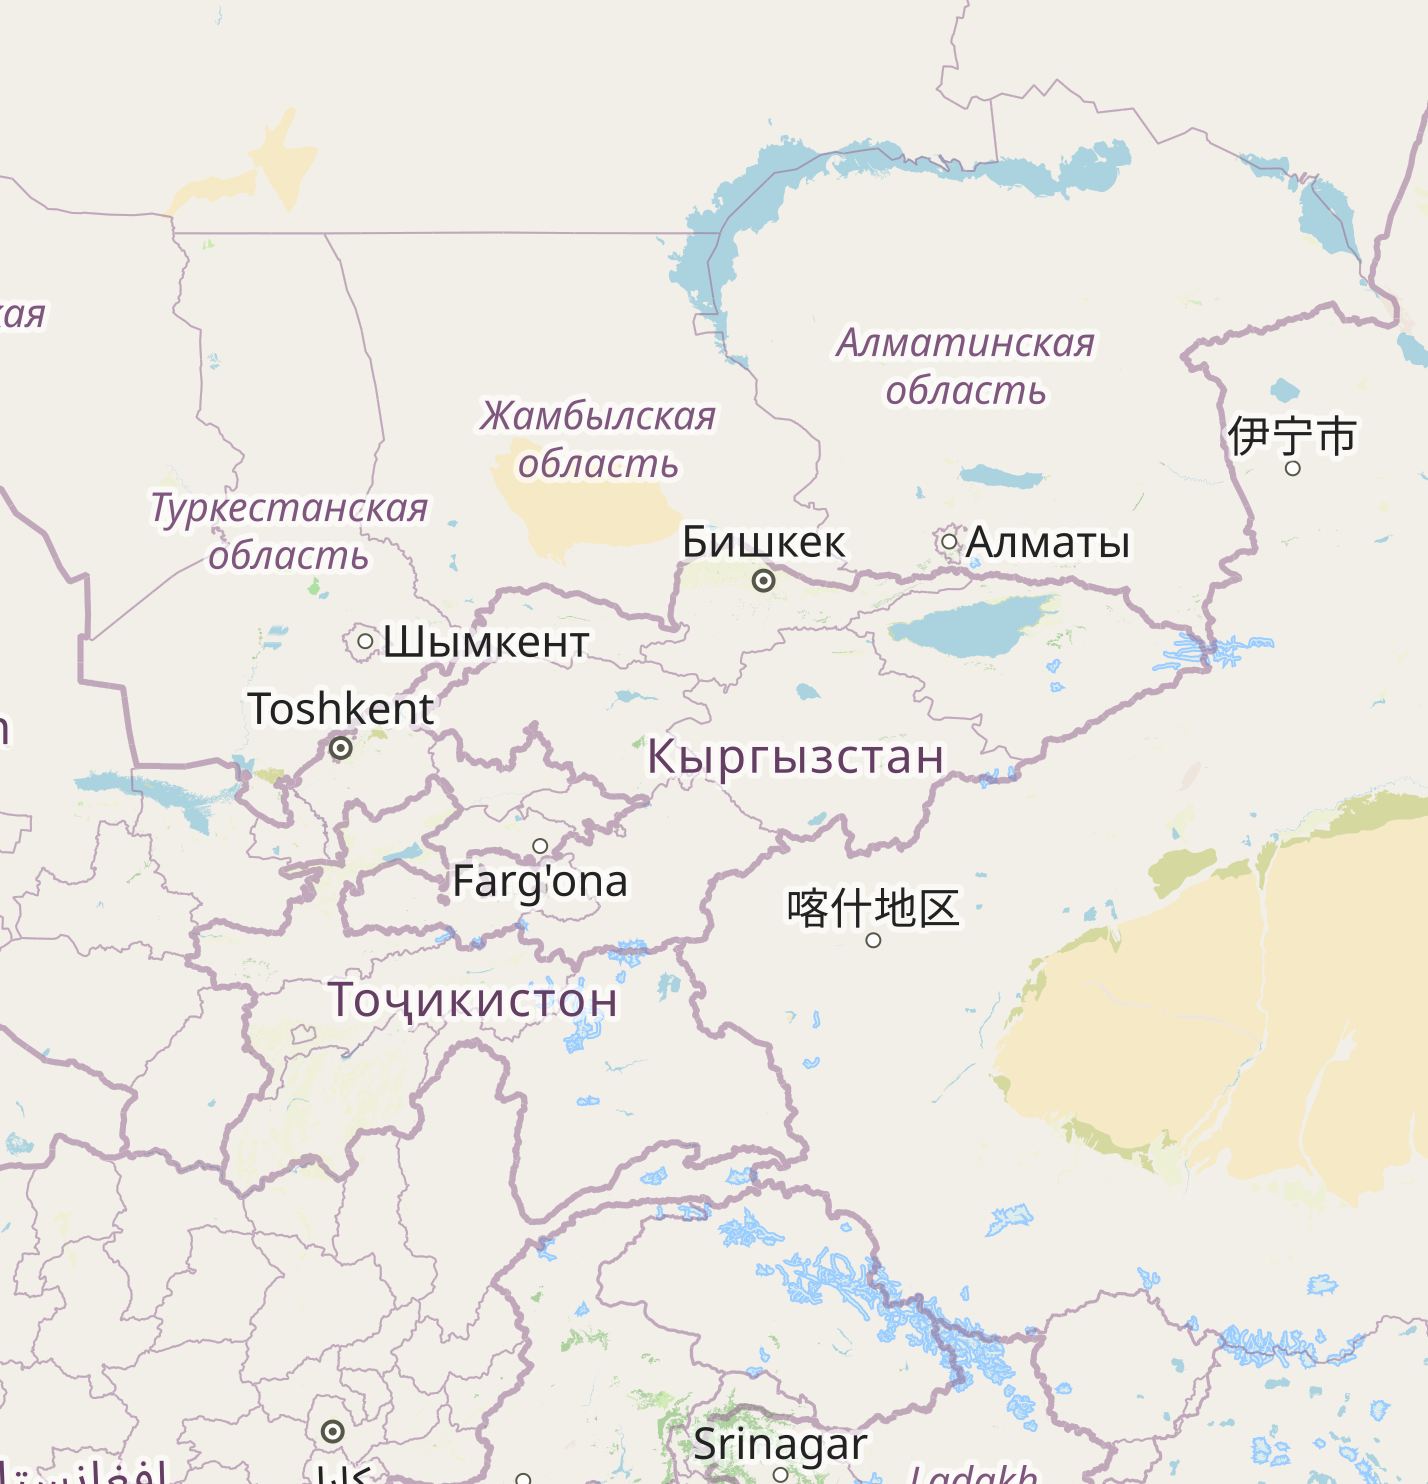
\includegraphics[width=0.7\textheight]{../graphics/map}}
        \caption{OpenStreetMap, 34\textdegree{}N to 48\textdegree{}N and 
            65\textdegree{}E to 83\textdegree{}E}
        \label{map}
    \end{figure}
\end{frame}

\begin{frame}{What is the data format?}
    \begin{itemize}
        \item files are in NetCDF format (Network Common Data Form), stores
            multi--dimensional arrays
        \item is a data format and set of libraries \cite{netcdf}
        \item libraries exists for C, Java, Fortran, Python, ... 
            \cite{netcdf-facts}
        \item full M2I3NPASM file (1 day) is 1.1 GB in size \cite{data-readme},
            our selection (\figref{map}) is about $6$ MB
        \item has 4 dimensions and 14 variables
        \item also includes metadata
    \end{itemize}
\end{frame}

\section{Building an Application}

\begin{frame}{Libraries I}
    \begin{itemize}
        \item I am working with Python, thus I need a Python library
        \item NetCDF library for netCDF4 available \cite{netcdf4}
        \item maintained by the NetCDF developers
        \item very popular library
        \item table below lists all required libraries
    \end{itemize}
\end{frame}

\begin{frame}{Libraries II}
    \center
    \begin{tabular}{| l | l | l |}\hline
        Name        & Reference         & Purpose\\\hline\hline
        PyQt5       & \cite{pyqt}       & GUI, threading\\\hline
        os          & \cite{py-os}      & working with directories\\\hline
        numpy       & \cite{py-numpy}   & saving data and 
                                \\&&manipulating arrays\\\hline
        pandas      & \cite{pandas}     & exporting data, 
                                        \\&&creating date series\\\hline
        json        & \cite{py-json}    & JSON files\\\hline
        datetime    & \cite{py-datetime}& working with dates\\\hline
        textwrap    & \cite{py-textwrap}& wrapping text\\\hline
        math        & \cite{py-math}    & testing for NaN\\\hline
    \end{tabular}
\end{frame}

\begin{frame}{Libraries III}
    \center
    \begin{tabular}{| l | l | l |}\hline
        Name        & Reference         & Purpose\\\hline\hline
        cartopy     & \cite{py-cartopy} & maps, borders \\\hline
        matplotlib  & \cite{py-mpl}     & plots, saving plots\\\hline
        netCDF4     & \cite{netcdf4}    & netCDF files\\\hline
        pathlib     & \cite{pathlib}    & file paths\\\hline
        re          & \cite{py-re}      & regular expressions\\\hline
        webbrowser  & \cite{browser}    & open a web page in browser\\\hline
        sys         & \cite{py-sys}     & pass arguments\\\hline
        warnings    & \cite{warnings}   & ignoring warnings\\\hline
    \end{tabular}
\end{frame}

\section{The Program}

\begin{frame}{Program requirements}
    \begin{itemize}
        \item netCDF data files (preferably M2I3NPASM)
        \item properly set up environment (see section 4.1 of my report)
        \item code for my program
            \href{https://github.com/moritz-konarski/internship}{here} or 
            upon request
    \end{itemize}
\end{frame}

\begin{frame}[fragile]{Demonstration}
    \begin{itemize}
        \item if the demonstration succeeded, go to Plot Results
        \item if it failed, continue here
    \end{itemize}
\end{frame}

\section{Demonstration}

\begin{frame}{Data processor I}
\begin{figure}
    \center
    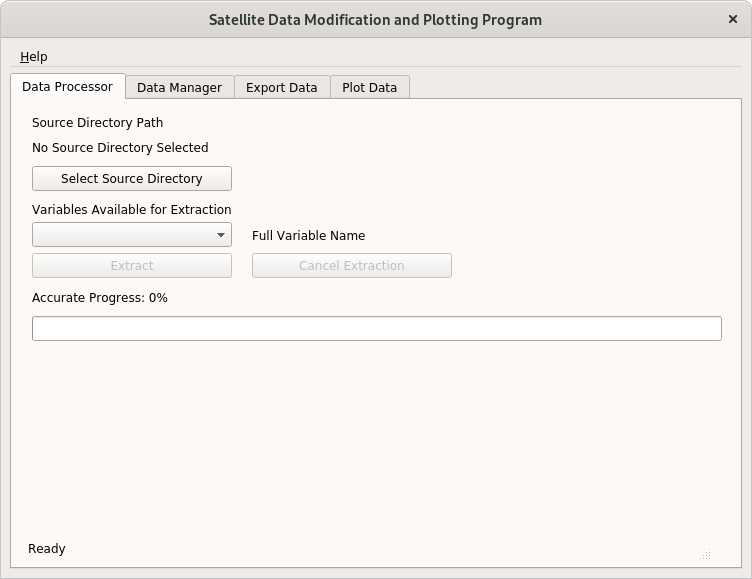
\includegraphics[width=0.95\textwidth]{../graphics/dp01}
    \vspace{-8pt}
    \caption{The Data Processor Tab}
\end{figure}
\end{frame}

\begin{frame}{Data processor II}
\begin{figure}
    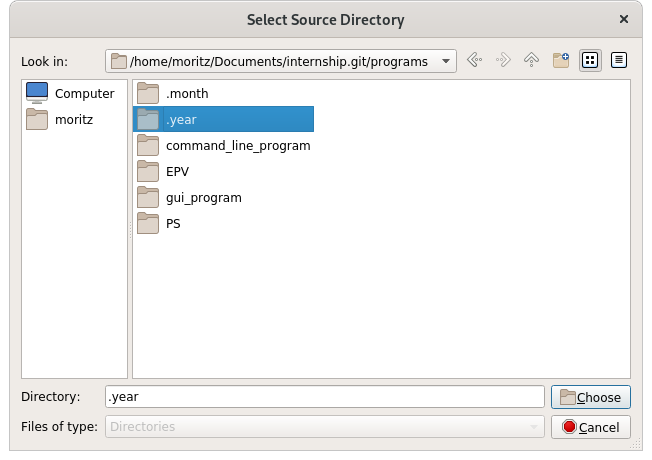
\includegraphics[width=0.95\textwidth]{../graphics/dp02}
    \vspace{-8pt}
    \caption{The Source Directory Selection Popup}
\end{figure}
\end{frame}

\begin{frame}{Data processor III}
\begin{figure}
    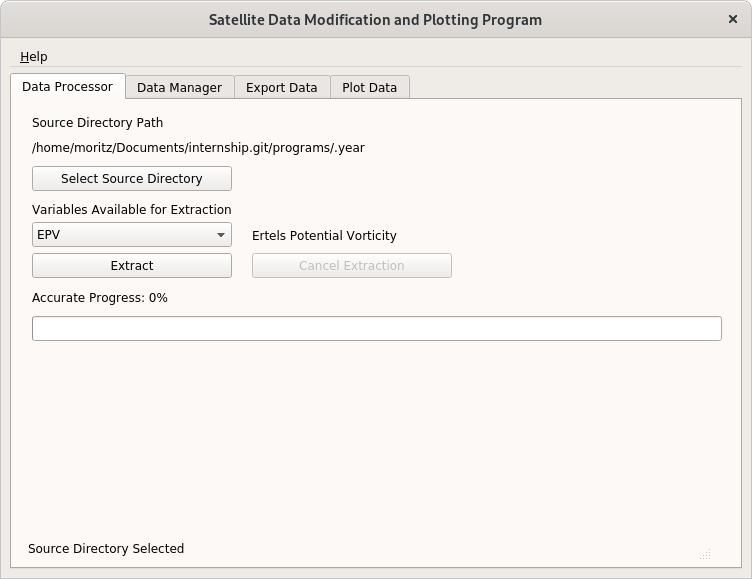
\includegraphics[width=0.95\textwidth]{../graphics/dp03}
    \vspace{-8pt}
    \caption{Data Processor with loaded source Directory}
\end{figure}
\end{frame}

\begin{frame}{Data processor IV}
\begin{figure}
    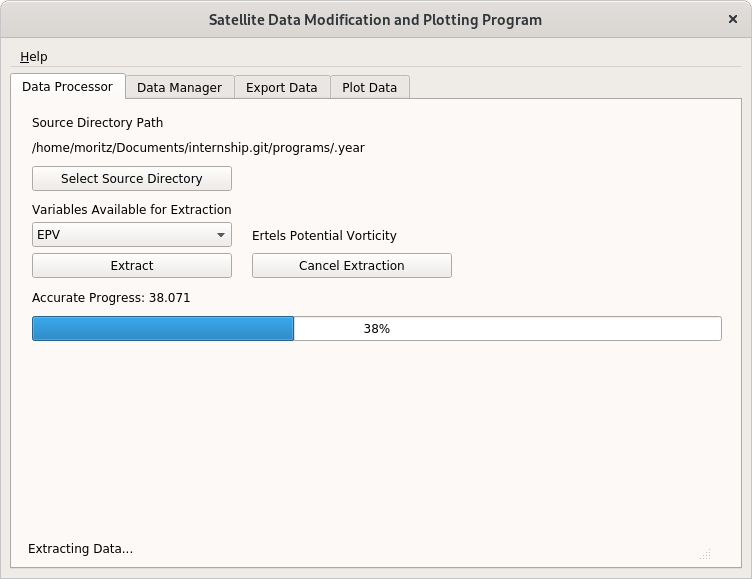
\includegraphics[width=0.95\textwidth]{../graphics/dp04}
    \vspace{-8pt}
    \caption{Extraction in Progress}
\end{figure}
\end{frame}

\begin{frame}{Data manager I}
\begin{figure}
    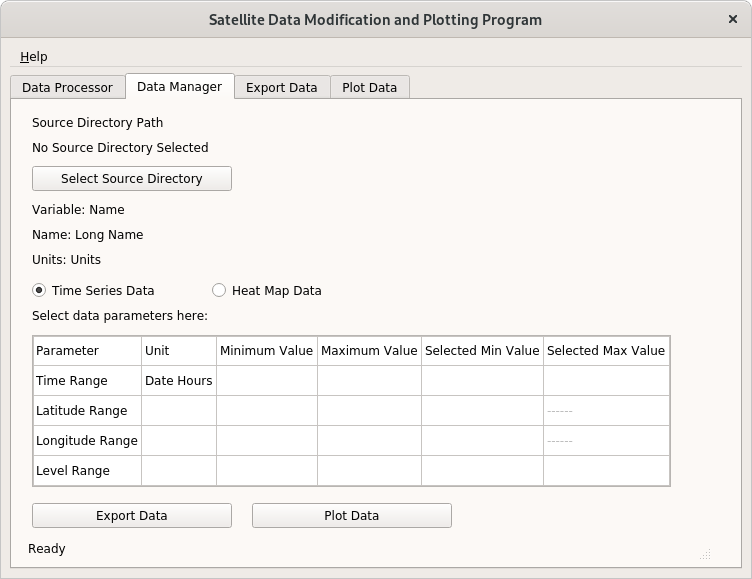
\includegraphics[width=0.95\textwidth]{../graphics/dm01}
    \vspace{-8pt}
    \caption{The Data Manager Tab}
\end{figure}
\end{frame}

\begin{frame}{Data manager II}
\begin{figure}
    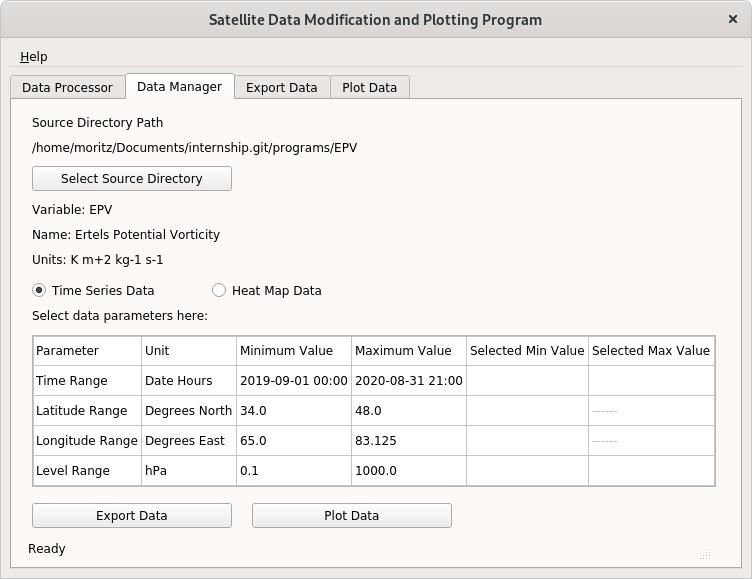
\includegraphics[width=0.95\textwidth]{../graphics/dm02}
    \vspace{-8pt}
    \caption{Data Manager with loaded Directory}
\end{figure}
\end{frame}

\begin{frame}{Data manager III}
\begin{figure}
    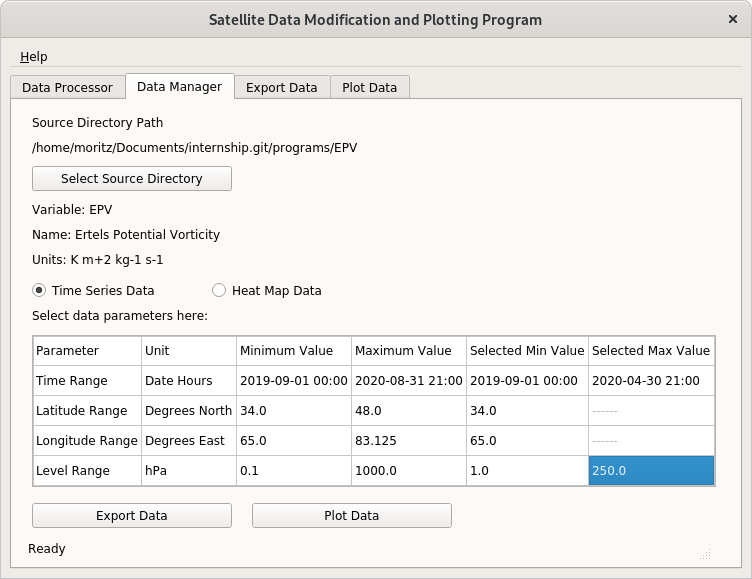
\includegraphics[width=0.95\textwidth]{../graphics/dm03}
    \vspace{-8pt}
    \caption{Data Manager in Time Series Mode}
\end{figure}
\end{frame}

\begin{frame}{Data manager IV}
\begin{figure}
    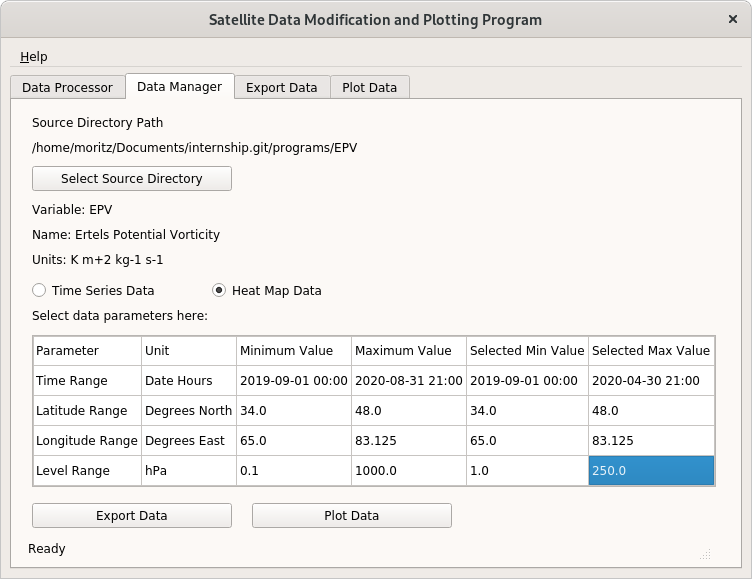
\includegraphics[width=0.95\textwidth]{../graphics/dm04}
    \vspace{-8pt}
    \caption{Data Manager in Heat Map Mode}
\end{figure}
\end{frame}

\begin{frame}{Data manager V}
\begin{figure}
    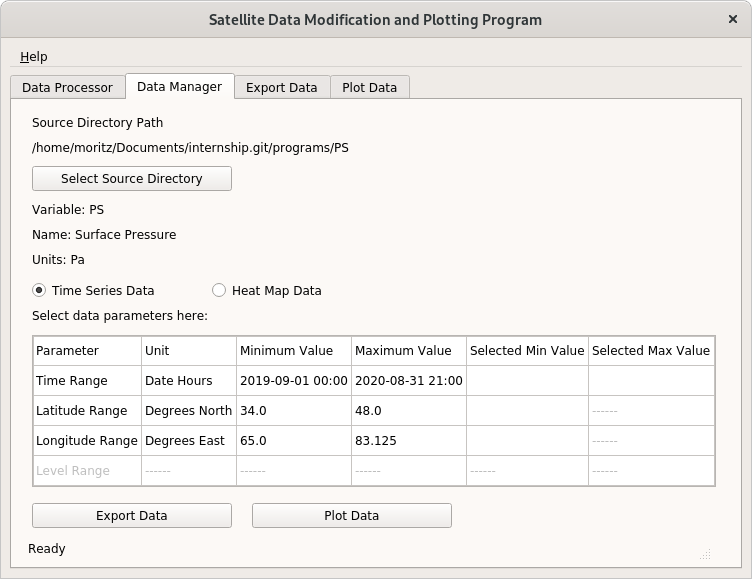
\includegraphics[width=0.95\textwidth]{../graphics/dm05}
    \vspace{-8pt}
    \caption{Data Manager with data without level}
\end{figure}
\end{frame}

\begin{frame}{Data exporter I}
\begin{figure}
    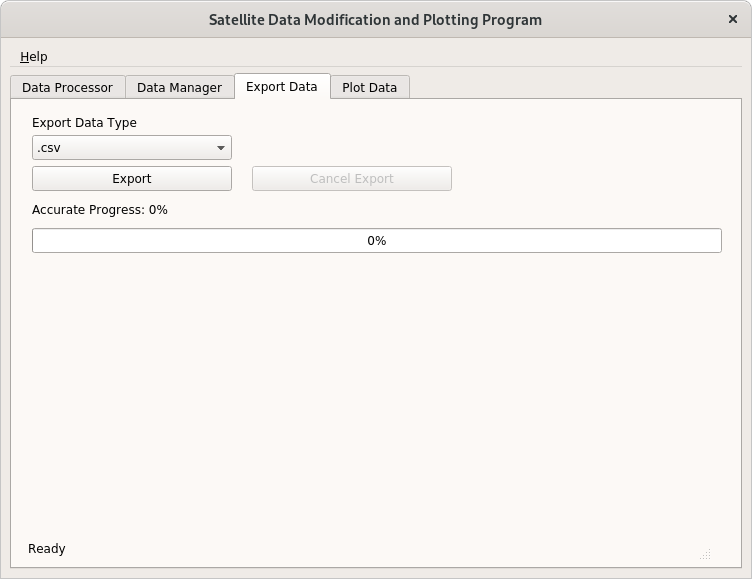
\includegraphics[width=0.95\textwidth]{../graphics/de01}
    \vspace{-8pt}
    \caption{The Data Export Tab}
\end{figure}
\end{frame}

\begin{frame}{Data exporter II}
\begin{figure}
    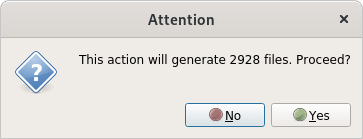
\includegraphics[width=0.5\textwidth]{../graphics/de02}
    \vspace{-8pt}
    \caption{The File Number Warning Message}
\end{figure}
\end{frame}

\begin{frame}{Data exporter III}
\begin{figure}
    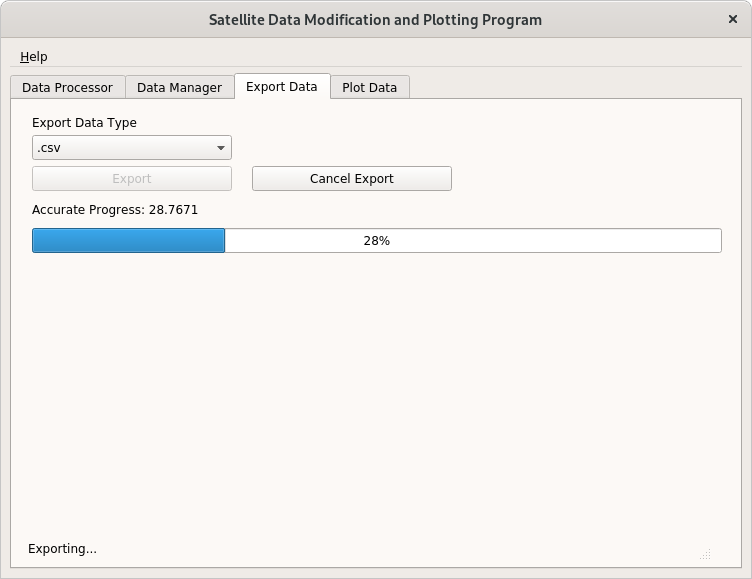
\includegraphics[width=0.95\textwidth]{../graphics/de03}
    \vspace{-8pt}
    \caption{Data Export in progress}
\end{figure}
\end{frame}

\begin{frame}{Data exporter IV}
\center
    Example of exported temperature data (in Kelvin) \\
    250 hPa, (34\textdegree{}N, 65\textdegree{}E)\\
    \vspace{5pt}
\begin{tabular}{| l | r |} \hline
    2019-09-01 00:00:00   &  237.30182  \\\hline 
    2019-09-01 03:00:00   &  236.86859  \\\hline
    2019-09-01 06:00:00   &  236.79724  \\\hline
    2019-09-01 09:00:00   &  236.82132  \\\hline
    2019-09-01 12:00:00   &  237.73062  \\\hline
    2019-09-01 15:00:00   &  238.40472  \\\hline
    2019-09-01 18:00:00   &  238.4401   \\\hline
    2019-09-01 21:00:00   &  238.20715  \\\hline
    2019-09-02 00:00:00   &  237.49396  \\\hline
\end{tabular}
\end{frame}

\begin{frame}{Data plotter I}
\begin{figure}
    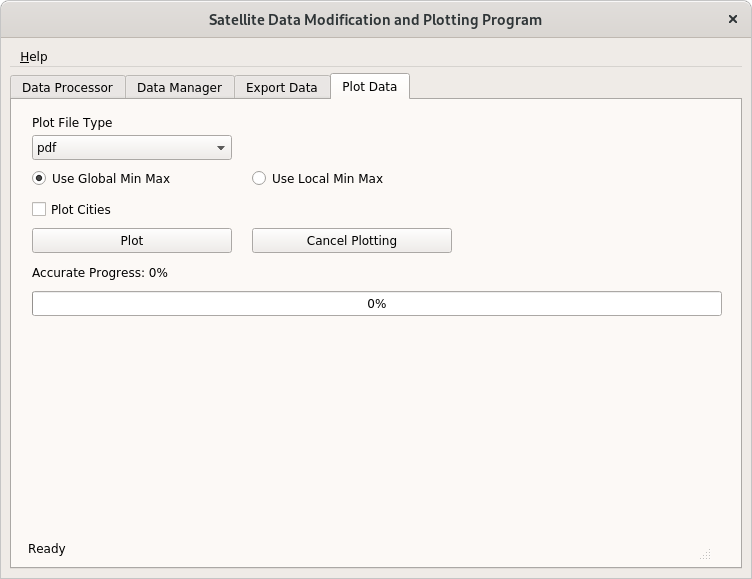
\includegraphics[width=0.95\textwidth]{../graphics/dpl01}
    \vspace{-8pt}
    \caption{The Data Plotter Tab for Heat Map Data}
\end{figure}
\end{frame}

\begin{frame}{Data plotter II}
\begin{figure}
    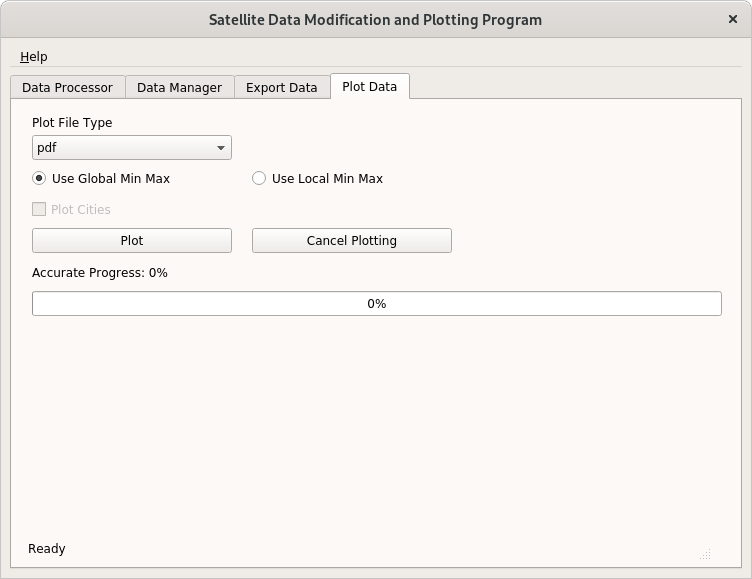
\includegraphics[width=0.95\textwidth]{../graphics/dpl02}
    \vspace{-8pt}
    \caption{The Data Plotter Tab for Time Series Data}
\end{figure}
\end{frame}

\begin{frame}{Data plotter III}
\begin{figure}
    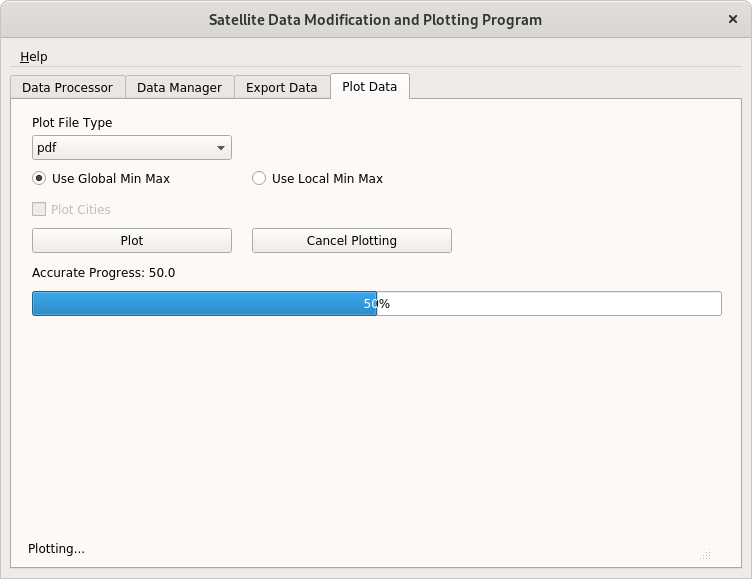
\includegraphics[width=0.95\textwidth]{../graphics/dpl03}
    \vspace{-8pt}
    \caption{Data Plotter in Progress}
\end{figure}
\end{frame}

\begin{frame}{Help website}
\begin{figure}
    \center
    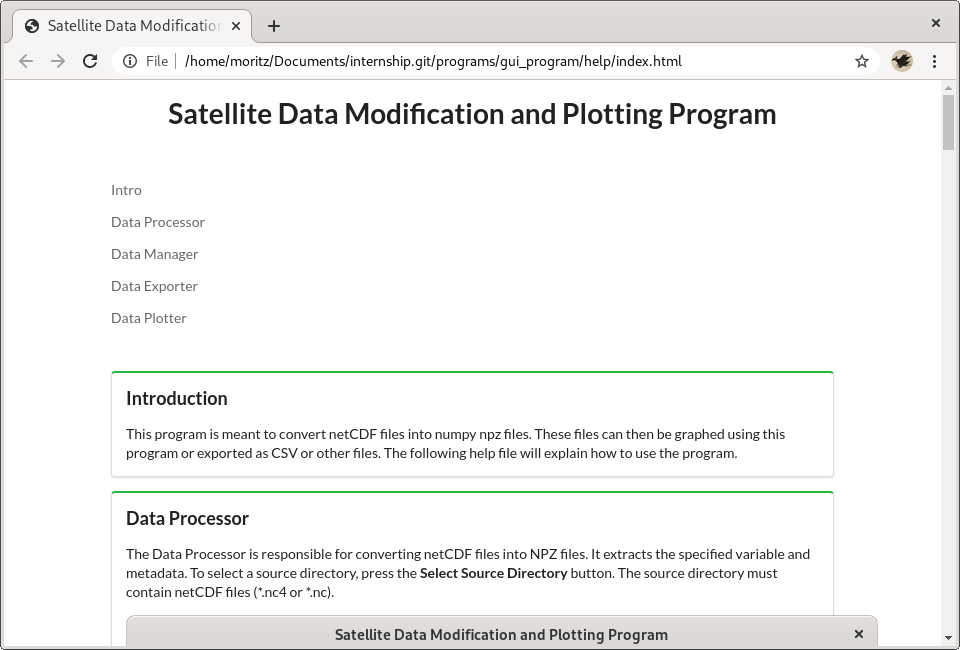
\includegraphics[width=0.95\textwidth]{../graphics/help}
    \vspace{-8pt}
    \caption{Screen Shot the Help section}
\end{figure}
\end{frame}

\section{Plot Results}

\begin{frame}{Temperature time series}
\begin{figure}
    \fbox{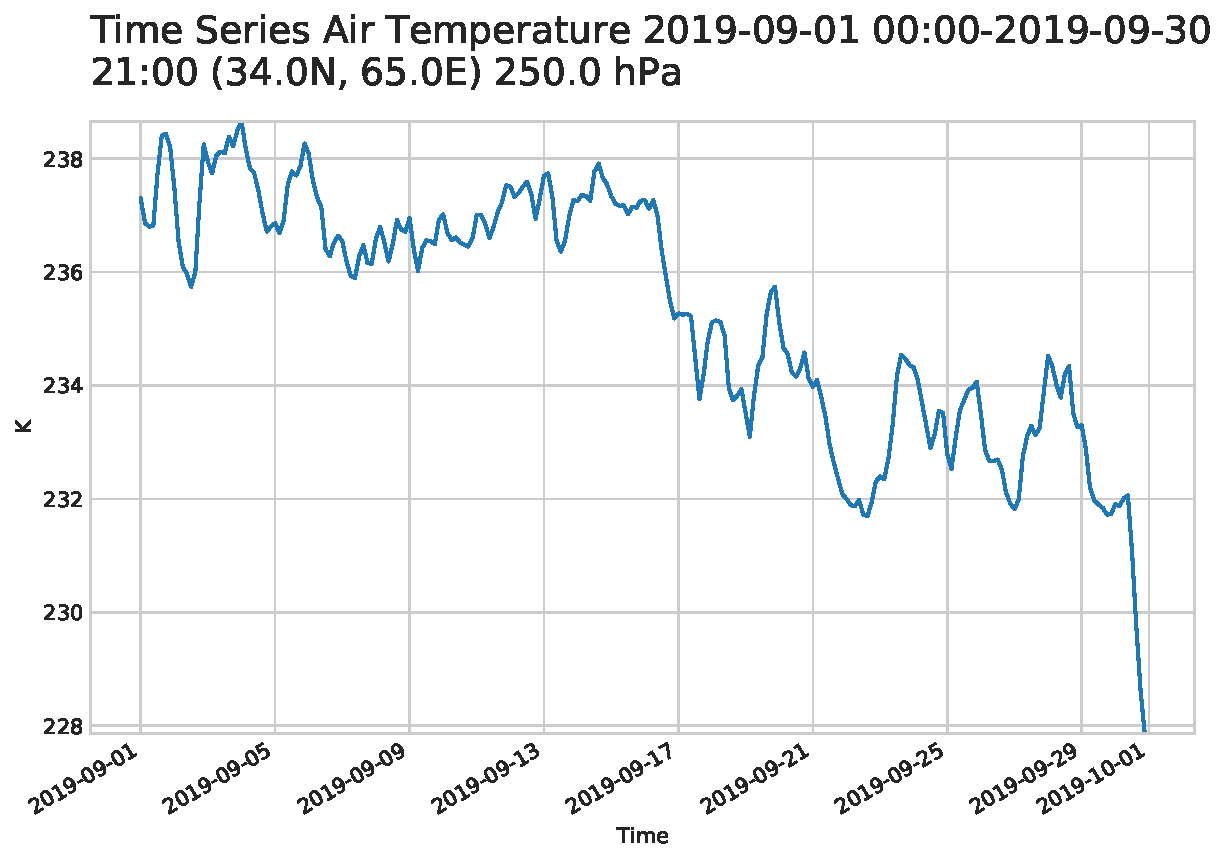
\includegraphics[width=0.95\textwidth]{../graphics/plt01}}
    \vspace{-6pt}
    \caption{Time Series Plot for Air Temperature in Kelvin ($K$)}
\end{figure}
\end{frame}

\begin{frame}{Temperature heat map I}
\begin{figure}
    \fbox{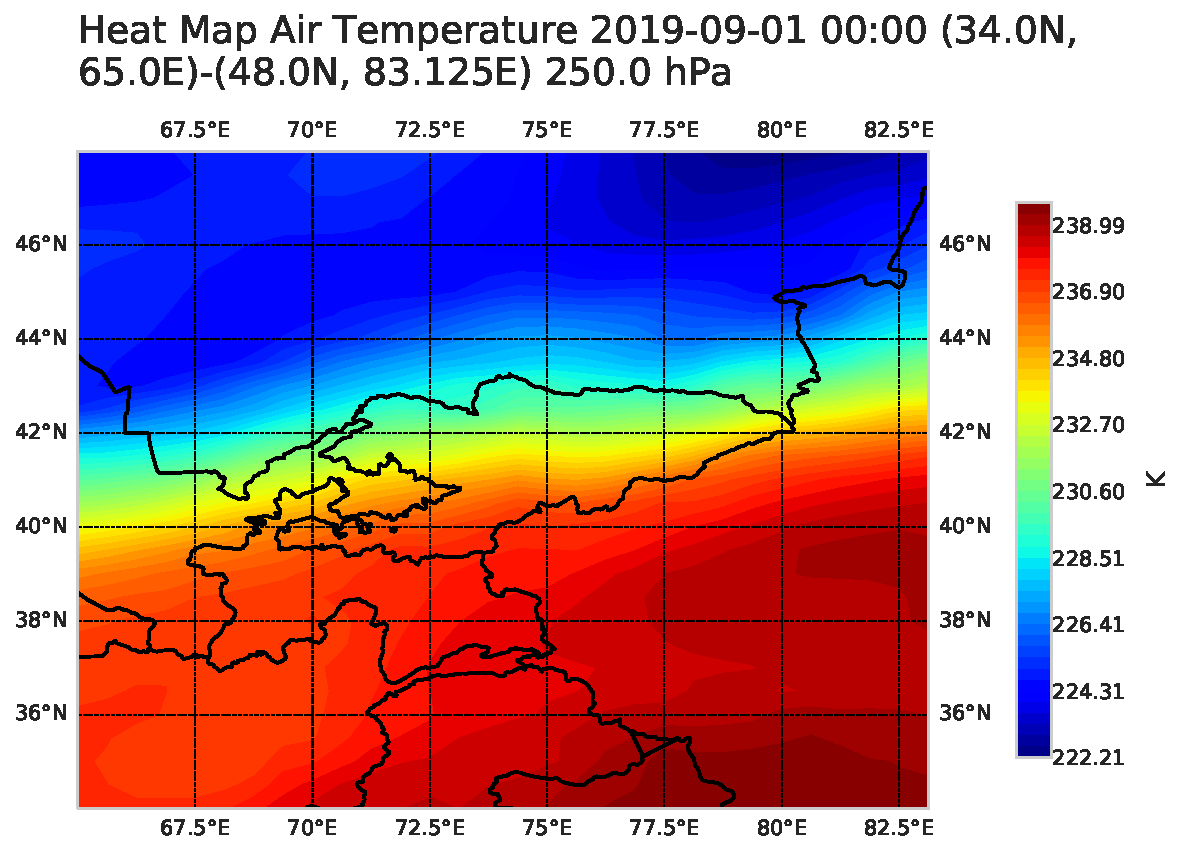
\includegraphics[width=0.95\textwidth]{../graphics/plt02}}
    \vspace{-6pt}
    \caption{Heat Map Plot for Air Temperature in Kelvin ($K$)}
\end{figure}
\end{frame}

\begin{frame}{Temperature heat map II}
\begin{figure}
    \fbox{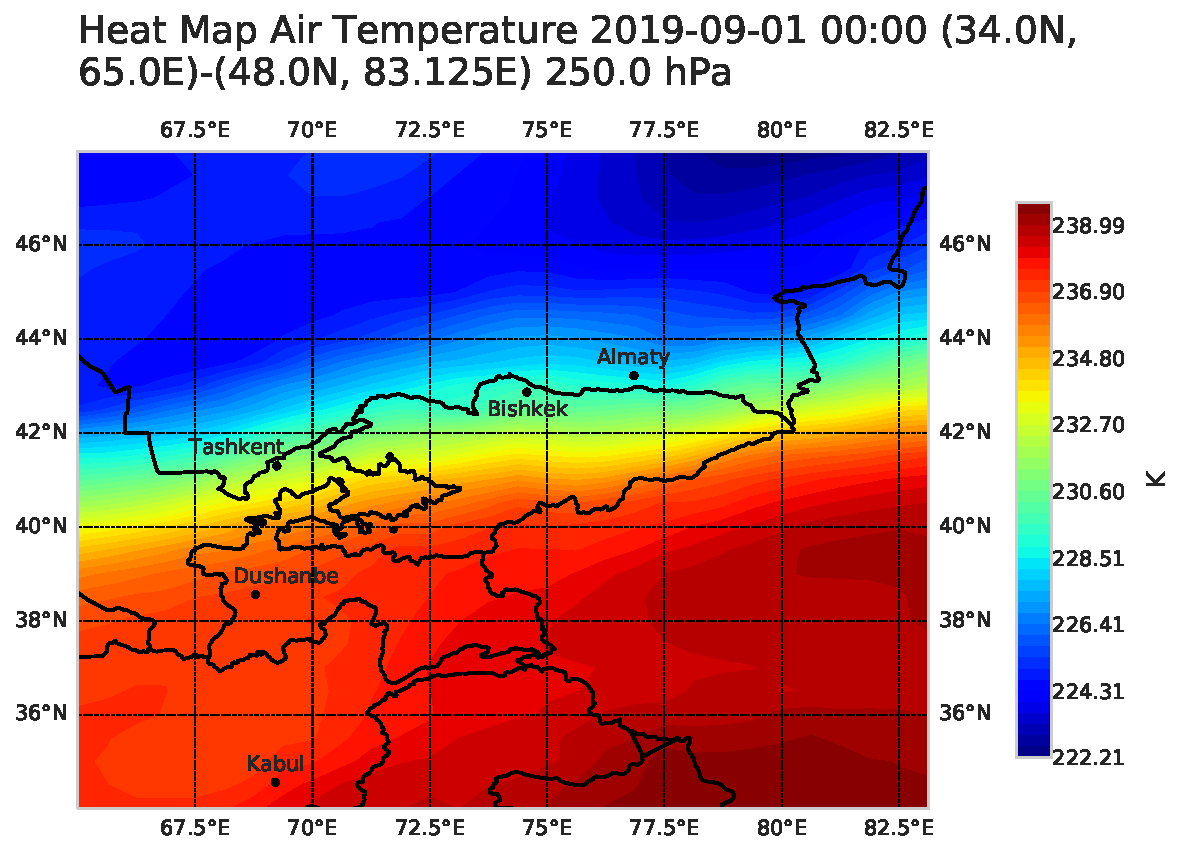
\includegraphics[width=0.95\textwidth]{../graphics/plt03}}
    \vspace{-7pt}
    \caption{Heat Map Plot for Air Temperature in Kelvin ($K$) with Cities}
\end{figure}
\end{frame}

\section{Data Investigation}

\begin{frame}{Purpose}
    \begin{itemize}
        \item use my program and gained skills 
        \item investigate temperature structure of the troposphere, temperature
            inversion around the tropopause
    \end{itemize}
\end{frame}

\begin{frame}{Troposphere}
    \begin{itemize}
        \item lowest layer of atmosphere
        \item up to about 12km above surface
        \item temperature at top about -63\textdegree{}C or 210K 
            \cite{tropopause}
        \item pressure is 1000 hPa to 200 hPa \cite{pressure}
    \end{itemize}
\end{frame}

\begin{frame}{Tropopause}
    \begin{itemize}
        \item boundary between troposphere and stratosphere
        \item demarcated by:
            \begin{enumerate}
                \item inversion of the temperature gradient \cite{tropopause}
                \item increase in potential vorticity (rotation of air masses)
                    \cite{tropopause}
                \item increase of ozone mixing ratio (how much ozone in the air
                    by mass or volume) \cite{atmosphere}
            \end{enumerate}
        \item to investigate: make plots of variable vs. pressure
        \item plot specifics: M2I3NPASM, 01.09.2019 at 12:00, 
            (40\textdegree{}N, 70\textdegree{}E)
    \end{itemize}
\end{frame}

\begin{frame}{Temperature}
\begin{figure}
    \fbox{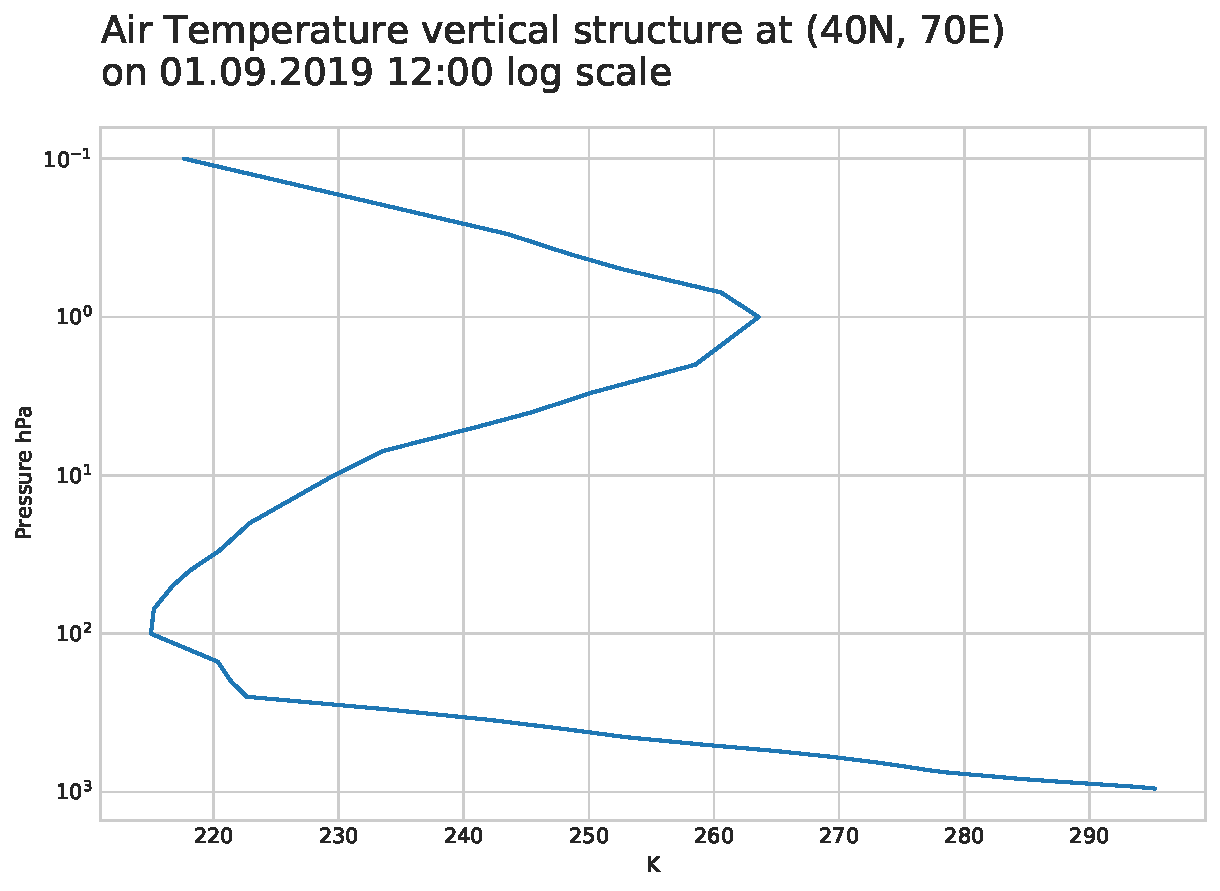
\includegraphics[width=0.95\textwidth]{../graphics/temperature}}
    \vspace{-7pt}
    \caption{Air Temperature by Air Pressure}
    \label{t}
\end{figure}
\end{frame}

\begin{frame}{Potential Vorticity}
\begin{figure}
    \fbox{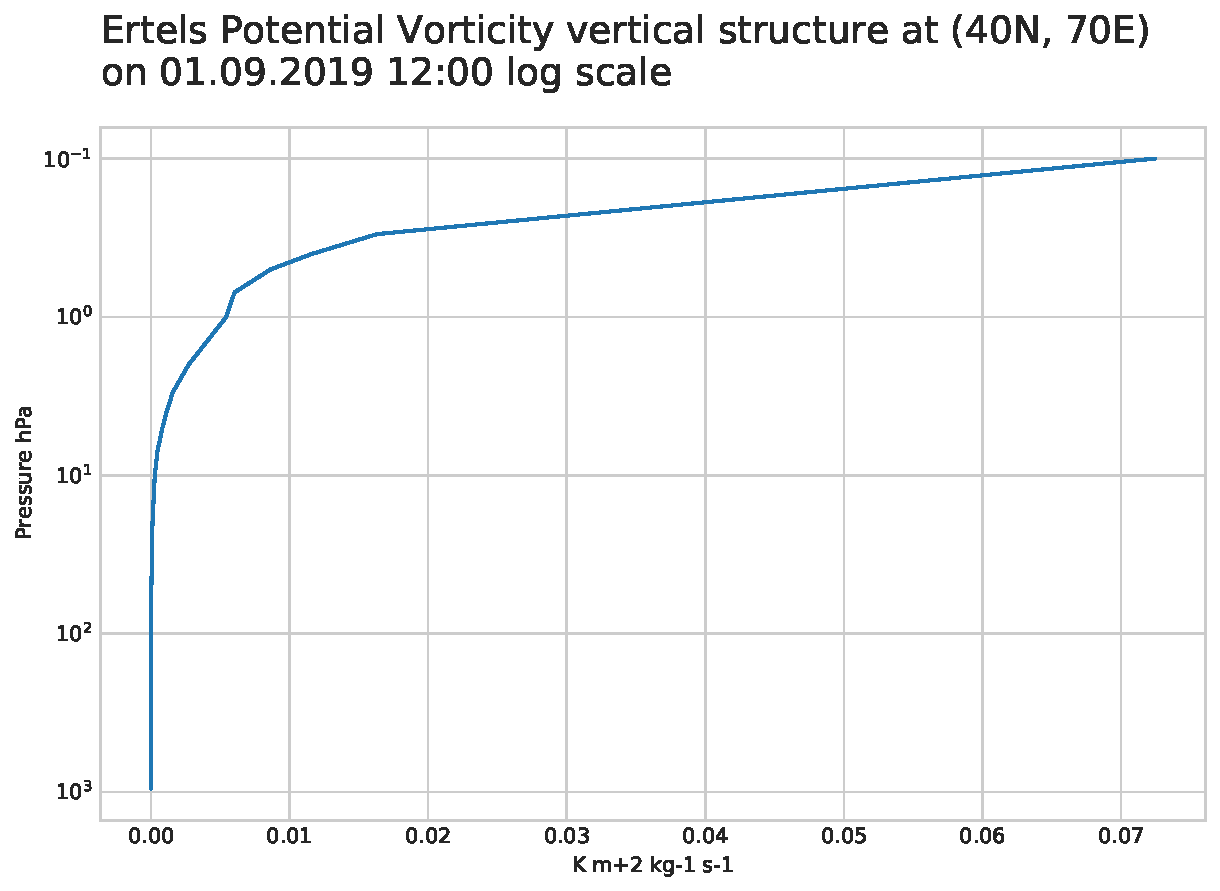
\includegraphics[width=0.95\textwidth]{../graphics/epv}}
    \vspace{-7pt}
    \caption{Ertel's Potential Vorticity by Air Pressure}
    \label{epv}
\end{figure}
\end{frame}

\begin{frame}{Ozone Mixing}
\begin{figure}
    \fbox{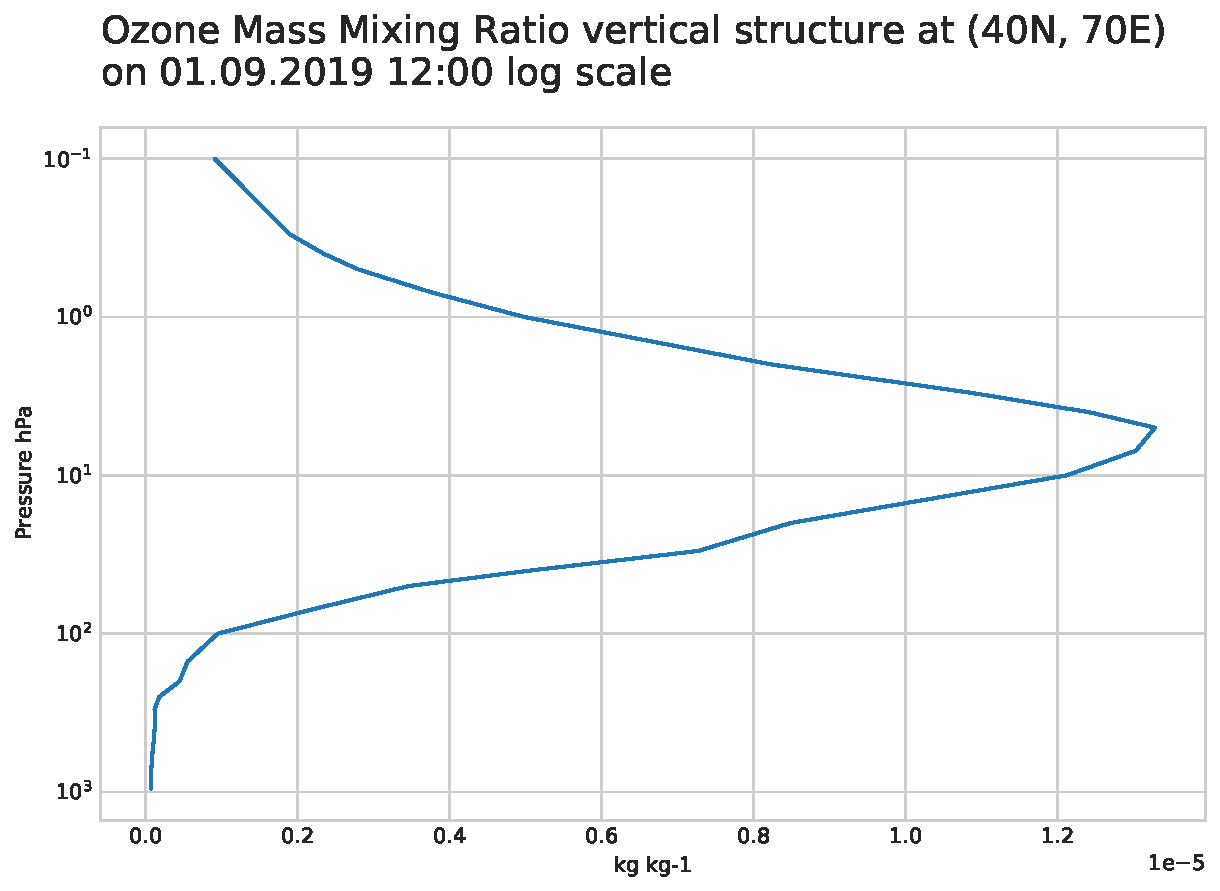
\includegraphics[width=0.95\textwidth]{../graphics/ozone}}
    \vspace{-7pt}
    \caption{Ozone Mass Mixing Ratio by Air Pressure}
    \label{ozone}
\end{figure}
\end{frame}

\begin{frame}{Results}
    \begin{itemize}
        \item tropopause temperature inversion in \figref{t} (caused by 
            aerosols and molecules) \cite{inversion} was in the right spot
        \item the ozone layer can be seen in \figref{ozone}
        \item the potential vorticity in \figref{epv} increased as expected
        \item the results obtained from the data analysis line up with the
            expected results
    \end{itemize}
\end{frame}

\section{Conclusion}

\begin{frame}{Conclusion}
    \begin{itemize}
        \item working with satellite data, GUI/Python development is valuable
        \item all skills I learned will be useful for my future, for jobs,
            further studies, or even research
    \end{itemize}
\end{frame}

\section{Q and A}

\tiny
\begin{frame}[allowframebreaks]{References}
    \bibliographystyle{abbrv}
    \bibliography{../src/bibliography}
\end{frame}

\end{document}
